\documentclass{article}
\usepackage[a4paper,total={170mm,257mm},left=15mm,right=15mm, top=20mm,bottom=25mm]{geometry}
\usepackage{amssymb}
\usepackage{amsmath}
\usepackage{graphicx}
\usepackage{subfigure}
\usepackage{hyperref}
\begin{document}
\begin{center}
	\LARGE \textbf{Machine Learning}\\
	\vspace{20pt}
\end{center}
\tableofcontents
% \vspace{40pt}
\large
\vfill
Things:
\begin{itemize}
	\item Every type of data in an element is called a \textit{feature}.
	\item Part of data that represents features is $X$, and the part which represents expected output is $y$.
	\item Number of elements in a dataset : $m$
	\item Number of features in an element: $n$
	\item $x_j^{(i)}$ is $j^{th}$ feature in $i^{th}$ element.
\end{itemize}
\pagebreak
\section{Linear Regression}
\subsection{Univariate Regression}
\begin{itemize}
	\item Process of fitting a straight line through 2D data, i.e. $n=1$.
	\item Proposed equation is of form $\theta_0 + \theta_1 x$. This is called a hypothesis. It is represented as
	\begin{align*}
		h_\theta(x)&=\theta_0 + \theta_1 x\\
		&= \begin{bmatrix}
			\theta_0 & \theta_1
		\end{bmatrix}
		\begin{bmatrix}
			1 \\x
		\end{bmatrix}\\
		&= \theta^T X
	\end{align*}
	Here, a $1$ is added to as a feature to make it easy to represent the constant term in matrix form.
	\item Ideally, $h_\theta(x_i)=y_i$ for $i=0$ to $m$. To represent how far the current hypothesis is from the best fit, a cost function is defined.
	$$J(\theta)= \frac{1}{2m} \sum_{i=1}^{m} (h_\theta(x^{(i)})-y^{(i)})^2$$
	This function, being quadratic, will be a parabola with a single global minima.
	\item To find the value of $\theta$ for which $J(\theta)$ is minimum, $\theta_j$ has to be chosen such that $\frac{\partial J(\theta)}{\partial \theta_j}=0$.
	\item For linear regression, $$\frac{\partial J(\theta)}{\partial \theta_j}=\frac{1}{m} \sum_{i=1}^{m} (h_\theta(x^{(i)})-y^{(i)})x_j^{(i)}$$
	\item So what is done is, these steps are repeated, $$\theta_0 = \theta_0 - \alpha * \frac{\partial J(\theta)}{\partial \theta_0}$$ and
	$$\theta_1 = \theta_1 - \alpha * \frac{\partial J(\theta)}{\partial \theta_1}$$ till the partial derivatives are below some thresholds.

	\item This technique is called as \emph{Gradient Descent}. This is a technique to find a \emph{local} minima, and not a global minima.
\end{itemize}
\subsection{Multivariate Regression}
\begin{itemize}
	\item In case of multivariate regression, data is $n$ dimensional. So the output parameter $y$ may be dependant on more than 1 $feature$.
	\item In this case, \begin{align*}
		h_\theta(X) &= \theta_0 + \theta_1 x_1 + \theta_2 x_2 \dots +\theta_n x_n\\
		&= \begin{bmatrix}
			\theta_0 & \theta_1&\theta_2&\dots&\theta_n
		\end{bmatrix}
		\begin{bmatrix}
			1 \\x_1 \\x_2 \\\vdots \\x_n
		\end{bmatrix}
		\\
		&= \theta^T X
	\end{align*}
	Where both $X$ and $\theta$ are vectors.
	\item Rest everything, $J(\theta)$, $\frac{\partial J(\theta)}{\partial \theta_j}$, gradient descent is same as linear regression.
\end{itemize}
\subsection{Polynomial Regression}
\begin{itemize}
	\item This is $same$ as multivariate regression, where the additional features are just higher degree versions of previous features.\\
	E.g. if $x_1=x$, then $x_2 = x^2$, $x_3=x^3$ etc.
	\item In this case, hypothesis might look like $h_\theta(X) = \theta_0 + \theta_1 x + \theta_2 x^2 \dots +\theta_n x^n$.
	\item This is useful if the data cannot be represented by a simple straight line.
\end{itemize}
\section{Logistic Regression}
Used for classifying the data into 2 or more classes.
\subsection{Classifying into 2 classes}
\begin{itemize}
	\item Here, y is a vector of 0s and 1s representing 2 classes. So, the hypothesis function should output a value between 0 and 1, which might be thought as probability of that element belonging to a class.
	\item If $h_\theta(X) > 0.5$, predict $y=1$, and otherwise $y=0$.
	\item To limit the hypothesis between 0 and 1, a sigmoid function is used. $$g(z) = \frac{1}{1+e^{-z}}$$
	As $z\rightarrow -\infty$, $g(z)\rightarrow 0$,\\
	as $z\rightarrow \infty$, $g(z)\rightarrow 1$,\\
	and $g(z)=0.5$ at $z=0$.
	\item Here, the hypothesis is represented as \begin{align*}
		h_\theta(X) &= g(\theta ^T X)\\
					&= \frac{1}{1+e^{-\theta ^T X}}
	\end{align*}
	\item $y=1$ is predicted if $h_\theta(X)>0.5$, i.e. $\theta^T X >0$, and $y=0$ if $\theta^T X \le 0$.
	\item Assume there are 2 features in the data, $x_1$ and $x_2$. $\theta^T X = \theta_0 + \theta_1x_1 + \theta_2x_2$. $y=1$ will be predicted if the point lies on e.g. left side of the line $\theta_0 + \theta_1x_1 + \theta_2x_2=0$, and $y=0$ if it lies on the other side.
	\item This line/curve $\theta^T X = 0$ is called $Decision\ Boundary$.
	\item If higher order features like $x_1^2$, $x_2^2$, $x_1x_2$ etc. are included, decision boundary can be parabolic/ circular/ elliptical etc.
	\item The cost function in this case, if wrote similar to that of linear regression, may not be convex i.e. it may have multiple local minima. This can be a problem since gradient descent is being used to optimize the parameters.
	\item So, the cost function for a single element is defined as \begin{equation*}
		Cost(h_\theta(X),y) = \left\{ \begin{array}{l}
			-log(h_\theta(X)) \ \ \ \ \ \ \ \ \ \text{if $y=1$}\\
			-log(1-h_\theta(X))\ \ \ \ \text{if $y=0$}\\
		\end{array}\right.
	\end{equation*}
	Here, if $y=1$, cost is $-log(h_\theta(X))$, which is 0 if $h_\theta(X)=1$, and tends to infinity if $h_\theta(X)=0$. Similarly for $y=0$.
	\item Cost function considering all elements is \begin{align*}
		J(\theta) &= \frac{1}{m} \sum_{i=0}^m Cost(h_\theta(X^{(i)}),y^{(i)})\\
		&= -\frac{1}{m} \sum_{i=0}^m y^{(i)}log(h_\theta(X^{(i)})) + (1-y^{(i)})log(1-h_\theta(X^{(i)}))
	\end{align*}
	\item For logistic regression as well, gradient of $J(\theta)$ comes out to be
	$$\frac{\partial J(\theta)}{\partial \theta_j}=\frac{1}{m} \sum_{i=1}^{m} (h_\theta(x^{(i)})-y^{(i)})x_j^{(i)}$$
	\item All $\theta_j$ parameters can be adjusted by using gradient descent in a similar way as linear regression.
\end{itemize}
\subsection{Multiclass classification}
\begin{itemize}
	\item If data is to be classified into more than 2 classes, a technique called one-vs-all is used.
	\item If there are $K$ classes, $K$ logistic regression models, $h^{(k)}_\theta(X)$ are trained.
	\item Value of  $h^{(k)}_\theta(X)$ represents the probability that an element belongs to class $k$.
	\item Class corresponding to maximum value of $h^{(k)}_\theta(X)$ is picked.
\end{itemize}
\section*{Regularization}
\begin{itemize}
	\item If there are too many features, and not many elements in the dataset, model may be too biased for the given dataset. It will fit the given points perfectly, but it'll fail to generalize, or it'll perform poorly on the test dataset. This problem is called as overfitting.
	\item To avoid this, some extra features can be manually removed, but it is hard to choose what features to keep and what to remove.
	\item Other method to remove this, is called regularization. For example, let's say the available dataset is approximately in a shape of parabola, but not exactly a parabola. So, we include quadratic, cubic, and $4^{th}$ degree terms.\\ This causes the model to overfit to the data.
	\item So, let's say we \emph{penalize} $\theta_3$ and $\theta_4$ by adding the terms $1000\theta_3 + 1000\theta_4$ to the cost function. This will result in bigger cost when either of $\theta_3$ or $\theta_4$ are big. So the values of coefficients of higher degree terms will automatically be less, which will result in less dramatic curve. This is less prone to overfitting.
	\item It's not always possible to choose the features to regularize, so as a convention, all parameters except $\theta_0$ are penalized.
	\item Cost function with regularization looks like :
	$$J(\theta)= \frac{1}{2m} \Bigg[\sum_{i=1}^{m} (h_\theta(x^{(i)})-y^{(i)})^2 + \lambda \sum_{j=1}^n \theta_j^2 \Bigg]$$
	\item For both linear and logistic regression,
	$$\frac{\partial J(\theta)}{\partial \theta_j}=\frac{1}{m} \sum_{i=1}^{m} (h_\theta(x^{(i)})-y^{(i)})x_j^{(i)} + \frac{\lambda}{m} \theta_j$$
	\item If value of $\lambda$ is set too large, $\theta_j\approx 0$ for $j=1$ to $n$. So, effective hypothesis will be\\ $h_\theta(X)=\theta_0$, which won't represent the data accurately either. This problem is called underfitting. Underfitting can also occur if there aren't enough features to fit the data properly.
\end{itemize}

\section{Neural Networks}
\begin{itemize}
	\item Many logistic regression model cascaded to eachother.
	\item A single logistic regression model can be thought of as a NN with $n$ units in the input layer, 0 hidden layers, and $K$ units in the output layer.
	\item These allow users to fit non-linear hypothesis without going for the polynomial features.
	\item Activation of unit $i$ in layer $l$ is represented by $a^{(l)}_i$.
	\item Matrix containing weights that map layer $l$ to layer $l+1$ is represented as $\Theta^{(l)}$.
	\item Vector of linear combinations of previous layer is denoted by $z^{(l)} = \Theta^{(l-1)} a^{(l-1)}$, and $a^{(l)}=g(z^{(l)})$.\\
	So, $a^{(2)}=g(\Theta^{(1)} X)$, $a^{(3)}=g(\Theta^{(1)} a^{(2)})$, and so on. In a 3 layer NN, $h_\Theta(X) = a^{(3)}$.
	\item In this case, $h_\Theta(X)$ is a vector of $K$ elements. $h_\Theta(X)_k$ represents $k^{th}$ element in that vector.
	\item Generally, an additional unit with activation 1 is added in every layer. It is called the bias unit.
	\item Cost function for NN is defined in a similar way as logistic regression.
	\begin{itemize}
		\item Cost of one single ($i^{th}$) element:
		\begin{equation*}
			cost^{(i)} = -\sum_{k=1}^K y^{(i)}_klog(h_\theta(X^{(i)})_k) + (1-y^{(i)}_k)log(1-h_\theta(X^{(i)})_k)
		\end{equation*}
		\item Cost function for $m$ elements:
		\begin{align*}
			J(\Theta) &= \frac{1}{m} \sum_{i=1}^m cost^{(i)}\\
			J(\Theta) &= -\frac{1}{m} \sum_{i=1}^m \sum_{k=1}^K y^{(i)}_klog(h_\theta(X^{(i)})_k) + (1-y^{(i)}_k)log(1-h_\theta(X^{(i)})_k)\\
		\end{align*}
		\item Cost function with regularization:
		\begin{align*}
			J(\Theta) &= -\frac{1}{m} \sum_{i=1}^m \sum_{k=1}^K y^{(i)}_klog(h_\theta(X^{(i)})_k) + (1-y^{(i)}_k)log(1-h_\theta(X^{(i)})_k) + \frac{\lambda}{2m}\sum_{l=1}^L \sum_{i=1}^{n_{l+1}} \sum_{j=1}^{n_l} (\Theta^{(l)}_{ij})^2\\
		\end{align*}
	\end{itemize}
	\item To train this network, all $\frac{\partial J(\Theta)}{\partial \Theta^{(l)}_{ij}}$ are needed.
	\item To evaluate these gradients, a method called \emph{Back Propogation} is used.
	\item Some required notes:
	\begin{itemize}
		\item Find $\delta^{(l)}_j$ for every node, which may be thought of as error in activation for $j^{th}$ node in $l^{th}$ layer of network.
		\item $\delta^{(L)} = a^{(L)}- y = h_\Theta(X)-y$.\\Delta value for output layer is simply the difference between obtained output and expected output.
		\item $\delta^{(l)} = (\Theta^{(l)})^T \delta^{(l+1)}.*g'(z^{(l)})$\\Where $g'(z)$ is first derivative of the sigmoid function, $.*$ operator means element-wise multiplication of the elements.\begin{itemize}
			\item $g'(z^{(l)}) = a^{(l)}.*(1-a^{(l)})$
		\end{itemize}
		\item $\delta^{(1)}$ is not calculated, as error in input cannot be defined.
		\item $\frac{\partial J(\Theta)}{\partial \Theta^{(l)}_{ij}} = a_j^{(l)}*\delta_i^{(l+1)}$ for all elements.
	\end{itemize}
	\item These steps are followed:\begin{itemize}
		\item Set $\Delta^{(l)}_{ij}=0$ for all $l,i,j$.
		\item For all $m$ elements ($i$ denotes element number): \begin{itemize}
			\item set $a^{(1)}=x^{(i)}$.
			\item Forward propogate to find $a^{(l)}$ for $l=1,2,\dots,L$.
			\item Set $\delta^{(L)} = a^{(L)}- y^{(i)}$.
			\item Find $\delta^{(L-1)},\dots,\delta^{(2)}$, using $\delta^{(l)} = (\Theta^{(l)})^T \delta^{(l+1)}.*g'(z^{(l)})$.
			\item $\Delta^{(l)}_{ij}+=a_j^{(l)}*\delta_i^{(l+1)}$
		\end{itemize}
		\item $\frac{\partial J(\Theta)}{\partial \Theta^{(l)}_{ij}} = \frac{1}{m} \Delta^{(l)}_{ij} + \lambda \Theta^{(l)}_{ij}$\\$\lambda$ term is added for non bias units only, i.e. for $j\neq 0$.
	\end{itemize}
	\item For more info on backprop, refer \href{https://youtu.be/Ilg3gGewQ5U}{this,} and \href{https://youtu.be/tIeHLnjs5U8}{this}.
	\item In NN, all values of $\Theta$ parameters cannot be initialized to 0, or anything equal, as activations of different nodes in a layer is are linear combinations of activations of previous layer. Every node will be identical to every other node in that layer if all weights are equal. So, the weights need to be randomly initialized.
	\item \textbf{Gradient Checking:}\begin{itemize}
		\item Even after implementing backprop, it's a good practice to check if it is working correctly.
		\item To check, $$\frac{\partial J(\Theta)}{\partial \Theta} = \frac{J(\Theta-\epsilon)-J(\Theta-\epsilon)}{2\epsilon}$$ This is used.
	\item To check $\frac{\partial J(\Theta)}{\partial \Theta^{(l)}_{ij}}$, value of $\Theta^{(l)}_{ij}$ is changed by $\epsilon$, rest are left as they were. Cost is calculated with this new $\Theta$, and approximate gradient is calculated.
	\item If this approximate gradient matches the one calculated using backprop, it is implemented correctly.
	\item This method of calculating gradient is computationally very slow, that's why backprop is used.
	\end{itemize}
\end{itemize}
\section{Diagnosing Errors}
If a model is designed and trained, but it is not predicting the output as expected when new data is introduced to it, some changes need to be made. To decide the changes, there are some things that can be done.
\begin{itemize}
	\item A metric to evaluate how good a model is performing is necessary to determine if changes are required to the model.
	\item Error on training set is not a good metric as a model may overfit the training data, so the training error will be very less, but it'll perform poorly on other inputs. That's why dataset is divided into 2 parts, training set and a test set. Model is evaluated on the basis of error in test set.
	\item Error is just the cost of the function with $\lambda=0$. In classification problem, error can be the number of wrong predictions.
\end{itemize}
\subsection{Degree vs Error, $\lambda$ vs Error}
\begin{itemize}
	\item While designing a model, degree of the hypothesis has to be chosen. If it is too less, model may underfit the data. If it is too large, model may overfit the data. So, different models of varying degrees are trained, and their test set errors are calculated.
	\item If both training error and test set erros are plotted w.r.t. degree of the hypothesis, training error will decrease as degree increases, as model will fit the data more and more closely. But the test set error will decrease for some time, and then it'll start increasing because of overfitting. Degree for which test set error is minimum is chosen.
	\item However, test set error is no longer a good metric, as the degree of hypothesis is \emph{trained} using that dataset. So in practice, dataset is divided into 3 parts, training set, cross validation set, and test set. Degree of polynomial and the value of lambda are trained using cross validation set, and test set is purely for evaluation purpose.
	\item Similar thing can be done with the regularization parameter $\lambda$. For a model, if a training error and CV error vs $\lambda$ plot is plotted, training error will increase with increase in $\lambda$. And CV error will start decreasing, hit a minima, and then start increasing again. Previous and later high value of error corresponds to overfitting and underfitting respectively.
	\item {\textbf{Overfitting is called as high variance.}}
	\\{\textbf{Underfitting is called as high bias.}}
	\item Whether the model has high variance or bias can be figured out by looking at their training and CV errors.\begin{itemize}
		\item If $J_{CV}(\theta) \approx J_{train}(\theta)$, and both are high, that means model is performing poorly even on training data. This means the model is underfitting, i.e. has high bias.
		\item $J_{CV}(\theta) >> J_{train}(\theta)$ means model has fit the data properly, but it is not generalizing well. So, the model is overfitting, i.e. has high variance.
	\end{itemize}
	Depending on this, different parameters can be tweaked, and changes can be made.
\end{itemize}
\subsection{Learning Curves}
\begin{itemize}
	\item Plot of error w.r.t. number of elements in training set is called a learning curve.
	\item Generally, training error will increase with increasing $m$, as it becomes more and more difficult to fit all the points in given dataset.
	\item And CV error will decrease with increase in $m$, as model is able to capture the pattern better and better.
	\begin{figure}[h]
		\centering
		\subfigure[Underfitting]{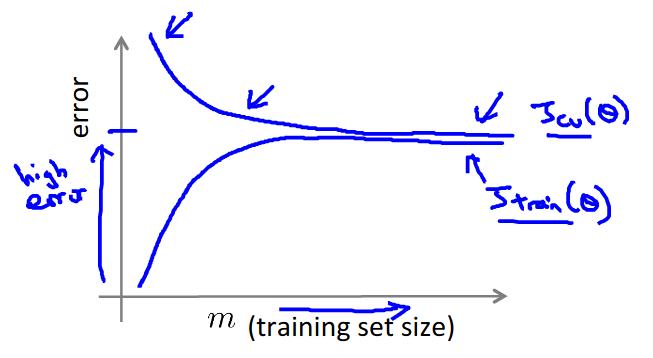
\includegraphics[scale=0.55]{im/LC_bias.png}}
		\subfigure[Overfitting]{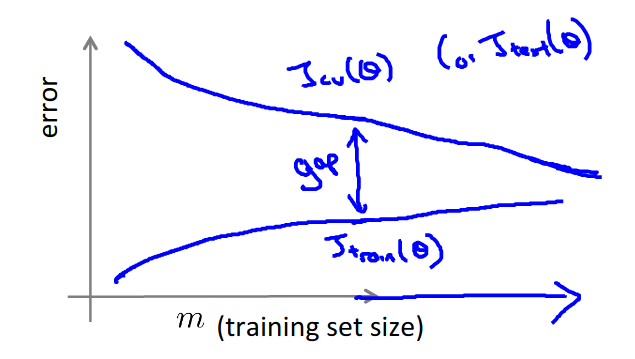
\includegraphics[scale=0.55]{im/LC_var.png}}
		\caption{Learning Curves}
		\label{}
	\end{figure}
	\item It can be seen from this figure that if a model is underfitting the data, getting more data is not going to help improve the performance, but in case of overfitting, using more training data may improve the model.
	\item Changes that can be done: \\\begin{tabular}{l c l}
	% \hline
	- Get more data for training set &\hspace{50pt} &to reduce overfitting\\
	- Try smaller set of features & &to reduce overfitting\\
	- Get additional features & &to reduce underfitting\\
	- Try adding polynomial features & &to reduce underfitting\\
	- Decrease $\lambda$ & &to reduce underfitting\\
	- Increase $\lambda$ & &to reduce overfitting\\
	% \hline
	\end{tabular}
	\item In NNs, having many hidden layers/ hidden units is equivalent of having many polynomial features. It is prone to overfitting.
	\item Similarly, having too few hidden layers/ hidden units may result in underfitting.
\end{itemize}

\section{Error Analysis}

\end{document}